\documentclass[a4paper, 12pt]{report} % \documentclass{} is the first command in any LaTeX code.  It is used to define what kind of document you are creating such as an article or a book, and begins the document preamble

\usepackage{graphicx} % package used to add images to the document
\usepackage{subcaption} %package used to create a figure of subfigures
\usepackage{tabularx} %package used to create tables that can fill the entire width of page
\usepackage{setspace} %package used to set the spacing between the lines.
\usepackage[table]{xcolor} % package used to color table rows and columns
\usepackage{fontspec} % package used to change the font of the document
\usepackage{fancyhdr} % package used to customize headers and footers
\usepackage{wrapfig} % used to wrap text around figures
\usepackage{tocloft} % used to add spaces before table of contents
\usepackage[sorting=none]{biblatex} % package used to add bibliographies
\usepackage[margin=1in]{geometry} % package used to change the margins



\setstretch{1.5} % setting the spacing between the lines to 1.5


\setmainfont{Times New Roman} % Set Times New Roman as the main font

% adding bibliographies here
\addbibresource{biblio.bib}
% images directory path for figures and logos
\graphicspath{ {./Images} }

% document metadata
\title{Simple Sample} % Sets article title
\author{Belal} % Sets authors name
\date{\today} % Sets date for date compiled

% includes section number in the figure and table number
\counterwithin{figure}{section}
\counterwithin{table}{section}

% remove chapter number from section number
\renewcommand{\thesection}{\arabic{section}}

% Customize page number position in the footer
\pagestyle{fancy} % need fancy page style for this to work
\renewcommand{\headrulewidth}{0pt} %removes fancy style added header line
\fancyhf{} % clears existing header/footer entries (default page numbering)
\fancyfoot[R]{\thepage} % sets page number on right side of the footer
\setcounter{tocdepth}{3}
\setcounter{secnumdepth}{3}
\begin{document} 
\setlength{\cftbeforetoctitleskip}{0pt plus 1pt} % sets the space before the table of contents to match sections
\setlength{\cftbeforeloftitleskip}{0pt plus 1pt} % sets the space before the list of figures to match sections
\setlength{\cftbeforelottitleskip}{0pt plus 1pt} % sets the space before the list of tables to match sections
    \begin{titlepage}
        \begin{center}
            
\includegraphics{Birzeit_Logo.png}

            Department of Computer Science 
            \vspace{0.8cm}

            Computer Security
            \vspace{0.8cm}
            
            \end{center}
            
            \textbf{\large{Title of Report:}}
            \vspace{0.4cm}
            
            \begin{center}
                \textbf{\Large{DDoS Attack Overview and Mitigation}}
            \end{center} 
            \vspace{0.8cm}
            
            \textbf{\large{Group Members with IDS:}}
            
            \hrulefill
            % \vspace{0.8cm}
            \begin{itemize}
                \item[$ $] BELAL HMEIDAT, 1202295 % removing order bullet to space
                \item[$ $] Moath HajAli, 1202862
                \item[$ $] Othman Hijawi, 1202927
            \end{itemize}
            

            \vspace{0.8cm}

            \textbf{\large{Supervisor:}}
            \vspace{0.4cm}
            
            \hspace{\parindent}MOHAMMAD ALKHANAFSEH %adding hspace same length as indentiation to force indent
            \pagebreak

    \end{titlepage}

    \pagenumbering{roman}
    \vspace{-0.8cm}
    \begin{abstract}
       Ever since the internet became openly available to everyone, cyber attacks have been a common occurrence that evolved in tandem with it. Nowadays the internet is integrated in people's daily lives more than ever, from personal devices, to servers that run the world's services, to IoT prephirals, the internet is everywhere and it will only get more integrated as time progresses. This fact made the cyberattacks very lucrative endeavour. One of the most common, effective, and hard to mitigate types of cyber attacks is DDoS or Distributed Denial of Service attack. Throughout the years DDoS attacks have evolved to be larger and more sophisticated. They are a natural flaw of the open internet that will always be present. This report will go into some more detail on DDoS background, damage it causes, its types and techniques it uses, vulnerabilities it exploits, what motivates it, and how to mitigate it. 
    \end{abstract}
    \pagebreak
    \tableofcontents
    \pagebreak
    \listoffigures
    \pagebreak
    \listoftables
    \pagebreak
    \pagenumbering{arabic}
    \counterwithin*{section}{part}
    \setcounter{page}{1}

    \section{Introduction}
        DDoS or Distributed Denial of Service constitutes a common type of cyber attack and a cyber crime that aims to make a network resource or service unavailable by flooding the network with fake requests from many different sources rendering it unreachable to legitimate users. The damage caused can be temporary or permanent. It works by flooding a network server traffic in an attempt to overwhelm it and exhaust its communication resources. DDoS attack is an evolution of DoS attack (Denial of Service attack) which also makes the server unavailable through fake or specialized faulty requests. DDoS attack akin to to a DoS attack, disables the availability of the system by sending faulty requests. Unlike DoS where the source of attack is a single point, DDoS attacks source of attack are many different points. This makes it harder to mitigate than DoS attacks as it is hard to block all sources of attack. These different sources of attack are called botnets or zombie networks. They are the sources that send fake traffic and operate on different devices from different IPs and geolocations. These botnets can run on legitimate user devices that were infected by a malware. The botnets have different families such as Agobot, SDBot, SpyBot, and GT Bot \cite{10.1007/978-0-387-44599-1_8} and each family can have many different variants. \cite{ddos_evolution}.
        DDoS attacks damage can be temporary or permanent. They might cause a vendor website to go down effectively causing them to lose a lot of sale profit for the whole period affected by the attack. They might bring down the servers of a whole company disabling it from providing services that can be critical. This is why it is important to understand such attack and how to mitigate it.
        DDoS attack has different types depending on the infrastructure it targets and the vulnerabilities it exploits. The most common types are volumetric, protocol, and application attacks. 
        DDoS attacks used by cyber criminals, hacktivists, and even governments to take down websites, services, and even whole networks. They are used to extort money, exert revenge, take down competition, or even take down a whole country's internet infrastructure.
        To mitigate DDoS attacks, different such as using firewalls, load balancers, and intrusion detection systems. These systems can detect and block fake traffic before it reaches the server. They can also detect and block botnets. There are also services that can be used to mitigate DDoS attacks such as Cloudflare, Akamai, and Arbor Networks. These services can detect and block fake traffic before it reaches the server. They can also detect and block botnets.

    \section{Background}
        \subsection{History of DoS and DDoS Attacks}
            DoS attacks have been around since the early days of the internet. Since then, there were many notable incidents involving DDoS. The first DoS attack was in 1974 when a student at the University of Illinois, David Dennis, sent fake requests to the ARPANET network. Morris Worm, 1988, was developed for research purposes but soon a bug caused the code to copy itself everywhere on the network resulting its developer Robert Morris a \$10,000 fine. DoS attacks were also common in 1991 when they were used to attack modern banks. Moreover, DoS had always been utilized in political conflicts since the early days of 1992 in the break up of Yugoslavia and the online intifada the following year \cite{history_of_ddos}.
            The year 1996 was the year is believed to be the year that had the first DDoS attack. It was on Panix, the third oldest ISP in the world \cite{wikipediaDenialofserviceAttack}. The attack was in the form of SYN flood attack, a type of DoS attack that works by sending the server a lot of SYN packets and thus leaves the server with many open ports awaiting ACK packets that never arrive \cite{syn_flood_attack}. It took 36 hours for Panix to recover and they responded with forming Security Trust Groups, anti-DDoS trust group of peers. This attack wasn’t officially a distributed attack though, because prior to the year 1999 all the DDoS attacks were done by having someone log into multiple systems to launch the attack rather than being automated and distributed across many devices. In 1999, Trinoo denial of service tool with remote command and control functionality using master slave setup. This tool causes massive UDP flood which once resulted in completely bringing down the internal network of the University of Minnesota by a Canadian teenager. These were the first attacks, then DDoS evolved to be more sophisticated and larger. In 2001, Code Red Worm attack combined both a worm and DDoS to attack Microsoft IIS web servers and it brought down the White House's website. One of the biggest DDoS attacks to this day \date{\today} was in 2018 on GitHub. It was a 1.35 Tbps attack that lasted for 10 minutes while the platform was unavailable for 5 minutes. Github was also hit in 2015 by a politicly motivated attack after the chinese search platform Baidu was infected and creating a botnet \cite{history_of_ddos}. It was mitigated by Akamai Prolexic service. In 2020, the biggest DDoS attack was on Amazon Web Services. It was a 2.3 Tbps attack that lasted for 3 days. It was mitigated by Arbor Networks service. Amazon's cloud computing division AWS recently experienced a sustained DDoS attack that appears to have lasted for around eight hours \cite{a10networksLargestReported}. AWS does offer its own DDoS mitigation service called Shield Advanced but it was unable to fully stop the attack. \cite{amazonManagedDDoS}.

        \subsection{Evolution of DDoS Attacks}
            DDoS attacks have evolved to be larger and more sophisticated. They have dramatically evolved from 200 Mbps \cite{ddos_evolution} of the aforementioned Code Red attack to the 2.3 Tpbs attack on AWS. They also became more sophisticated as the botnets used also evolved. In their paper about DDoS Evolution \cite{ddos_evolution}, Paul Barford and Vinod Yegneswaran talk about these botnets evolutions, namely evolution for SpyBots, GT Bot, SD Bot, and Agobot, from the architecture of the botnets, botnets control, botnets propagation mechanisms that they use to find new hosts to the techniques, vulnerabilities they exploit, malware delivery mechanisms, to deception mechanisms. 

            \begin{figure}[h!]
                \centering
                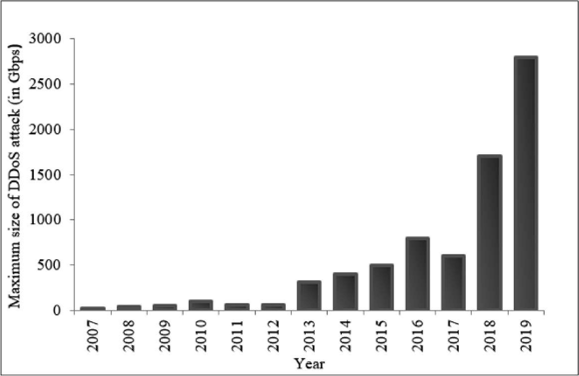
\includegraphics[width=0.8\textwidth]{Images/ddos_evolution.png}
                \caption{Number of DDoS Attacks over the years \cite{ebraryFundamentalsDDoS}}
                \label{fig:ddos_evolution}
            \end{figure}

            \subsection{Literature Review}

            \begin{spacing}{1}
                \begin{table}
                    \centering
                    \label{tab:litterature_review}
                    \caption{Literature Review}
                    \begin{tabularx}{\linewidth}{|p{2cm}|p{3cm}|X|}
                        \hline
                        \textbf{Author} & \textbf{Title} & \textbf{Summary} \\
                        \hline
                        \textbf{Paul Barford and Vinod Yegneswaran} & \textbf{An Inside Look at Botnets} \cite{10.1007/978-0-387-44599-1_8} & This article provided very detailed and valuable information about the different types of botnets, the architecture of the botnets, botnets control, botnets propagation mechanisms that they use to find new hosts to the techniques, vulnerabilities they exploit, malware delivery mechanisms, to deception mechanisms in addition to how they evolved.\\
                        \hline
                        \textbf{Pavithra, KC and Shetty, Snitha and Nagesh, HR} & \textbf{A comprehensive study of distributed denial of service attacks and defense mechanisms} \cite{pavithra2014comprehensive} & This paper presents a study on DDoS, its different types and the mechanisms used to prevent them. The authors classify these attacks based on the targeted protocol layers and discuss traditional and modern defense methods, anomaly detection and hybrid solutions. This paper emphasizes the need for automated defense mechanisms and highlights the importance of integrating machine learning techniques for effective and robust solutions. \\
                        \hline
                        \textbf{Mirkovic, J., Prier, G., Reiher} & \textbf{Attacking DDoS Attacks at the Source} \cite{1181418} & This paper focuses on strategies used to mitigate DDoS attacks by targeting the sources of malicious traffic. The authors propose a comprehensive framework to detect and stop DDoS attacks as close to their sources as possible. They discuss the implementation of tracking mechanisms to identify attack sources, the deployment of filtering techniques to block malicious traffic, and collaboration among ISPs to enhance the effectiveness of these measures. The study also explores the challenges associated with source-based mitigation, such as the possibility of false positives and the need to adopt broad-based defensive measures. The proposed solutions aim to reduce the impact of DDoS attacks by preventing malicious traffic from gathering and reaching the target. \\
                        \hline
                    \end{tabularx}
                \end{table}
            \end{spacing}


        \section{Types and Mechanisms}
        To prevent these attacks, we must understand and distinguish between the different types of denial of service attacks within the three main categories: volumetric, protocol, and application. However, some attacks fall outside these categories. Attackers may use a combination of techniques to make their attacks more sophisticated.
        Those three classifications contain dozens of DDoS attack types, such as UDP, ICMP, IP, TCP and HTTP flood attacks and their variants. We cover the categories and attack types in depth below.

        \subsection{Volumetric DDoS Attacks}
        Volumetric DDoS attacks attempt to flood resources so that requests overwhelm servers and traffic overwhelms networks and databases. They seek to saturate the bandwidth of the site under attack, and the size of the attack is usually measured in bits per second. Volumetric DDoS attacks include many different attacks, which we will mention below \cite{esecurityplanetCompleteGuide}.

        \subsubsection{UDP Flood Attacks}
        UDP does not create a two-way session, but rather sends packets of data without waiting for a response. This makes it ideal for flood attacks, which overwhelm a server with a large volume of UDP packets. The server must check each packet for an application, which exhausts and consumes its resources. Attackers target servers by sending packets to specific IP addresses and ports, overwhelming the server or network bandwidth.
        Specific UDP Flood Attacks can use:
        \begin{itemize}
            \item Domain Name Service (DNS).
            \item Network Time Protocol (NTP).
            \item Simple Service Discovery Protocol (SSDP).
            \item Media data such as audio or video packets.
            \item Voice over IP (VoIP) telephone packets.
            \item NetBIOS.
            \item Peer-to-peer (P2P) networks like BitTorrent or Kad packets.
            \item Simple Network Management Protocol (SNMP).
            \item Quote of the day (QOTD).
            \item Video game specific protocols like Quake and Steam.
            
        \end{itemize}

        Variants of the UDP Flood attack include:
        \begin{itemize}
            \item 
            \item \textbf{UDP Fragmentation Flood} This variation of the UDP Flood attack sends larger, but fragmented packets to the victim server. The server will attempt to assemble the unrelated, forged, and fragmented UDP packets and may become overwhelmed in the process.
            \item \textbf{Specific UDP Amplification Attacks} \\ Instead of using a large number of compromised devices, attackers can send a legitimate UDP request to a large number of legitimate servers with the victim server as a spoofed IP address. The responses from these legitimate servers suddenly overwhelms the targeted device. Protocols often used in amplification attacks include: NTP, SNMP, and SSDP.
            
        \end{itemize}


        \subsubsection{CharGEN Flood Attacks}
        It is an old protocol designed for testing and debugging. It creates a stream of random characters when receiving each request. In a CharGEN Flood attack, attackers exploit this protocol by sending a large number of requests to a server running this protocol. Each request creates a stream of random characters, which confuses the server and consumes its resources.

        \subsubsection{ICMP (Ping) Flood Attacks}
        The Internet Control Message Protocol consists of specific error messages and operational information commands sent between network devices such as Time Stamp, Time Exceeded error, Echo Request, and Echo Reply. Echo Request and Echo Reply combine to make the “ping” command.
        Attackers use a large number of devices to flood servers with spoofed Ping packets without waiting for replies. The protocol requires the server to receive the requests as well as respond to them which consumes both incoming and outgoing bandwidth.

        \subsubsection{ICMP Fragmentation Flood}
        A variant of the ICMP Flood attack, the ICMP Fragmentation Flood sends fragmented ICMP packets instead of fully formed commands. The victim server attempts to reconstruct valid commands from the spoofed ICMP packets and will exhaust resources attempting to make connections between intentionally unrelated fragments.

        \subsubsection{Malicious Application Attack}
        In misused application attacks, hackers exploit compromised high-traffic applications like P2P servers to redirect their traffic towards a victim server. Because the traffic originates from legitimate sources and uses properly formed packets, defensive systems often allow it, leading the victim server to be overwhelmed by the sudden surge in traffic \cite{impervaDDoSAttack}.


        \subsection{Protocol DDoS Attacks}
        Protocol-specific DDoS attacks exploit vulnerabilities in network protocols to overwhelm specific resources . Unlike volumetric attacks, which focus on volume, these attacks target protocol mechanisms, and  measured in packets per second.
        Examples of protocol DDoS attacks:
        \begin{enumerate}
        \item Null IP Attack: Attackers send packets with empty headers, causing server resources to be consumed.
        \item TCP Flood Attacks:
        \begin{itemize}
            \item SYN Flood: Floods servers with request packets (SYN), causing resources to be consumed while waiting for responses (ACK).
            \item SYN-ACK Flood: Sends fake (SYN-ACK) responses, causing server resources to be consumed.
            \item ACK Flood: Floods servers with fake (ACK) responses, causing resources to be consumed.
            \item ACK Fragmentation Flood: Uses fragmented packets to flood server memory during packet reassembly.
            \item RST/FIN Flood: Floods servers with fake RST or FIN packets to consume resources.
            \item Fake Multiple Session Flooding via ACK/RST/FIN: Sends multiple fake packets to simulate legitimate traffic and drain server resources.
            
            
        \end{itemize}
        \item Session Attacks: Uses legitimate TCP sessions from multiple bots to flood servers with empty sessions, consuming resources.
        \item Slowloris: Sends partial HTTP requests to servers to keep sessions open without closing, consuming resources.
        \item Ping of Death: Sends large IP packets that are too large for the receiver’s memory to hold, causing memory to crash when reassembled by the receiver.
        \item Smurf Attack: Sends fake (ICMP ping) requests to a network broadcast address, causing all devices on the network to respond and flooding the victim with responses.
        \item Fraggle Attack: Similar to Smurf but uses fake UDP packets.
        \item Low Orbit Ion Cannon (LOIC) and High Orbit Ion Cannon (HOIC): Tools used to flood targets with UDP, TCP, or HTTP packets, originally designed for stress testing, are being abused in DDoS attacks by attackers.
        \item 
        \end{enumerate}


        \subsection{Application Layer DDoS Attacks}
        Application DDoS attacks target vulnerabilities in Layer 7 applications to cause them to fail. Unlike other attacks that focus on infrastructure, these attacks overload application resources like CPUs and memory.

        Types of Application DDoS Attacks:
        
        \begin{itemize}
            \item GET Attacks: Botnets send numerous concurrent GET requests for large files.
            \item POST Attacks: Botnets send many concurrent POST requests containing large files for server storage.
            \item Low-and-Slow POST Attacks: Using tools like R.U.D.Y., attackers send HTTP POST requests slowly to evade detection by DDoS defenses.
            \item Single Session or Single Request Attack: Exploits HTTP 1.1 to include multiple requests within a single packet, evading packet-based defenses.
            \item Fragmented HTTP Flood: Botnets establish valid HTTP connections and send fragmented packets slowly to exhaust server resources.
            \item Recursive GET Flood: Overwhelms servers by requesting long lists of pages or images, mimicking legitimate browsing behavior.
            \item Random Recursive GET Flood: Variates requests to evade detection while consuming server resources.
        \end{itemize}

        These attacks exploit vulnerabilities in application software to disrupt services by overloading resources or causing application failures.

        \subsection{Other DDoS Attacks}
        While volume, protocol, and application attacks are the most common forms of DDoS attacks, there are other types:

            \subsubsection{Advanced Persistent DoS (APDoS)}
            A type of attack that hackers use to cause significant damage. These attacks involve a variety of patterns such as HTTP flooding and SYN flooding, and regularly target attack vectors that send millions of requests per second. APDoS attacks can sometimes last for weeks, thanks to hackers’ ability to quickly change their tactics and implement strategies to evade security defenses.

            \subsubsection{Multi-vector attacks}
            Attackers can execute multiple simultaneous attacks to increase the impact of a DDoS attack, for example, they can use volumetric attacks to distract while simultaneously executing HTTP flood attacks from different low-bandwidth botnets.

            \subsubsection{Zero-day DDoS attacks}
            These attacks occur when attackers discover new vulnerabilities in applications, protocols, or devices and quickly execute a DDoS attack before service providers can patch them.

            \subsection{Botnets}
            In addition to the different types of attacks and vulnerabilities used, DDoS attacks also differ in the Botnet Types
            \begin{spacing}{1}
                
                \begin{table}[h!]
                    \centering
                    \caption{Summary of Different Botnet Types in DDoS}
                    \label{tab:botnet_summary}
                    \begin{tabularx}{\textwidth}{|X|X|X|X|X|X|}
                        \hline
                        \textbf{Botnet Type} & \textbf{Purpose} & \textbf{Architecture} & \textbf{Control Mechanisms} & \textbf{Propagation} & \textbf{DDoS Capabilities} \\
                        \hline
                        \textbf{SpyBots} & Primarily used for information theft and espionage. Can also perform DDoS attacks. & Centralized C\&C architecture with a modular design. & Initially IRC-based, later versions use HTTP for stealth. & Exploits software vulnerabilities and uses social engineering. & Can be used to flood targets with traffic, although not primarily designed for DDoS. \\
                        \hline
                        \textbf{GT Bot} & Designed for launching DDoS attacks and other basic malicious activities. & Script-based, often using mIRC script, lightweight, and easy to deploy. & IRC-based C\&C for real-time communication. & Scans networks for vulnerabilities and uses weak passwords for infiltration. & Commonly used for large-scale DDoS attacks due to ease of deployment and control. \\
                        \hline
                        \textbf{SD Bot} & Versatile botnet capable of various malicious activities including DDoS. & Modular framework, cross-platform compatibility. & Uses both IRC and HTTP for command and control. & Exploits vulnerabilities and uses brute force attacks on FTP and SSH. & Can conduct DDoS attacks while also performing spamming and phishing. \\
                        \hline
                        \textbf{Agobot} & Highly sophisticated and versatile, used for a wide range of malicious activities including DDoS. & Highly modular, written in C++ with an object-oriented design. & Supports multiple C\&C protocols including IRC, HTTP, and P2P. & Exploits various vulnerabilities in Windows services. & Known for its robust DDoS capabilities, can perform both volumetric and application layer attacks. \\
                        \hline
                    \end{tabularx}
                    
                \end{table}
                
            \end{spacing}    

        \section{Threats and Risks}
            The DDoS attack can expose a huge risk to the target, because it is very easy and inexpensive to execute and they can cost an organization millions of dollars in costs, lost revenue, lost productivity, loss of market share, and a huge problem to the brand’s reputation. Also, the attack can cause severe resource exhaustion, mitigation complexity, complex attribution, and service disruption by attacking the application layer instead of the network layer like most attacks \cite{radwareShieldSquareCaptcha}.
            
                \begin{itemize}
                    \item \textbf{Resource Exhaustion}  An application layer DDoS attack drains the servers memory, CPU, and bandwidth. This affects response times and overall performance.

                    \item \textbf{Mitigation Complexity} Unlike network-based attacks, application layer attacks require specialized defenses that inspect application-level traffic.

                    \item \textbf{Complex Attribution}  Identifying the true source of these attacks is challenging due to spoofed IP addresses and botnets.

                    \item \textbf{Service Disruption}  Critical services like web applications, email, and VOIP become unusable during attacks.

                \end{itemize}

                These could all very much be a very serious risk that a DDoS attack can expose, ultimately, DDoS attacks can be short, or long-lasting. Obviously, long-lasting attacks can be more costly, but it’s important to not underestimate the damage that shorter attacks can incur, especially if they are recurrent. Following are the main threats that can affect an organization by a DDoS attack \cite{corero}:

                \begin{itemize}
                    \item \textbf{Loss of revenue} Downtime can be extremely costly, depending on the type of business and the size of the organization. One hour of downtime for a financial institution versus an hour of downtime for a university network may incur very different costs, but the impact on customers or users is significant in either case. 

                    \item \textbf{Loss of productivity}  When a business application or service is degraded or taken offline completely, that usually means employees can’t work as efficiently, or in many cases, at all. 

                    \item \textbf{Redemption costs} Exhausting resources to rebuild after a DDoS attack means additional labor costs like overtime, and the fallout can affect the company’s public relations, and overwork the customer support teams who will be panicking to respond to customer complaints or requests


                    \item \textbf{Damage to brand reputation}  Some industries such as gaming, hosting, data centers, and financial services rely heavily on their reputation for service availability. If customers can’t trust that a vendor will be consistently online and available, they can easily spread the word online, via Google Reviews or other social media channels. To acquire new customers in a highly competitive market a company must maintain a positive reputation.
                    \item \textbf{Loss of market share}  DDoS attacks can create customer churn. When an end user is denied access to Internet-facing applications, or if latency issues obstruct the user experience, it can impact the bottom line, because customers who can’t rely on a company to provide consistent service may go elsewhere to conduct their business.

                    \item \textbf{Random Costs}  Attackers threaten an organization by holding their files hostage and threatening to launch a DDoS attack on top of that unless the organization pays a handsome number of bitcoin ransom fee. Sometimes companies pay the ransom because it is better to have the situation taken care of right away without any public attention.

                \end{itemize}
                

                \section{Counter Measures and Mitigation}
                    As much as DDoS attacks might seem unpleasant, it is important to realize that there is no way for these types of attacks to simply go away. The reality is that these attacks will stay as there are interconnected networks. Generally, there are two levels of attacks that DDoS does, Infrastructure Attacks and Application Attacks. At a high level, a denial of service attack can fall into two categories according to the level of the OSI model at which it functions \cite{a10networksDDoSAttack}.
                    
                    An Infrastructure attacks target vulnerabilities or weaknesses in the network layer or the transport layer. Most DDoS attacks fall into this category, including SYN flood, Ping of Death (PoD), ICMP flood, and UDP flood attacks. Depending on the specific tactics used, infrastructure attacks can be further subdivided into volumetric attacks and protocol attacks.Also, there are volumetric attacks which the most common type of denial of service attack they focus on flooding the victim’s server or bandwidth with false requests to render it unable to accept regular traffic. Protocol attacks target the protocols used in transferring data to crash a system.

                    On the other hand, application attacks work at the application layer to target weaknesses in a specific application to render it unable to communicate or deliver content. This most often occurs through the HTTP protocol, and less commonly using FTP, NTP, SMTP, or DNS. Unlike volumetric infrastructure attacks, application attacks can achieve their intended impact with a relatively low volume of requests, making them particularly difficult to detect. 
                    Before diving into the ways someone can detect an attack, best practices to mitigate it, and how to combat it, it is important to understand the motives behind such attacks. 

                    \subsection{Motives}
                    Attackers can have many motivations when initiating a DDoS attack, some do it for revenge on a certain person or an organization who they believe did something bad to them while others use DDoS attacks for blackmail, which is basically demanding money to stop the attack and restore the normal operations. Competition is another important motive, where businesses try to damage their rivals to gain an advantage. Hacktivists, who are activists using hacking to promote their cause, also perform DDoS attacks that make people more aware of social or political issues.
                    
                    \subsection{Detection}
                        Knowing that a DDoS attack is occurring is the first step in mitigating or preventing one. In order for us to identify an attack, we have to collect a huge amount of network traffic data and then perform analysis on this data to determine if the traffic is friendly or hostile, this process can be carried out automatically or manually. DDoS detection is essential for promptly neutralizing attacks but two requirements must be satisfied for this to occur, the quickness of detecting the attack, and the precision in identifying it \cite{kentikDDoSDetection}.

                        Some of the main symptoms that we can notice when analyzing huge chunks of data are as follows:

                        \begin{itemize}
                            \item An unusual number of traffic originating from a single IP address or IP range
                            \item A lot of traffic from clients who share a single behavioral profile, such as device type, geolocation, or web browser version.
                            \item An unexplained surge in requests to a single page or endpoint.
                            \item Odd traffic patterns such as spikes at odd hours of the day or patterns that appear to be unnatural.

                        \end{itemize}

                        There are two primary means of detecting DDoS attacks: in-line examination of all packets and out-of-band detection via traffic flow record analysis. Either approach can be deployed on-premises or via cloud services. The basic in-line DDoS detection capabilities of network devices such as load balancers, firewalls or intrusion prevention systems may have once provided acceptable detection when DDoS attacks were smaller but high-volume attacks can overwhelm these devices, since they utilize memory-intensive stateful examination methods.

                        Dedicated DDoS mitigation appliances are the primary way to accomplish in-line detection (and remediation) today. They can become costly and have a short life cycle in the face of higher volume threats. These appliances are still necessary and relevant for mitigation because ASIC and network processor power is needed for deep packet inspection when scrubbing traffic but for cost-effectiveness and scaling reasons, moving detection out of mitigation devices has become the norm.

                        Out-of-band DDoS detection is accomplished by a process that receives flow data from NetFlow, J-Flow, sFlow, and IPFIX-enabled routers and switches, then analyzes that flow data to detect attacks. Mitigation of the attacks is then triggered manually or automatically, via routing or appliance-based methods.

                    \subsection{Prevention}

                    To reduce the risk of a devastating denial of service attack, organizations need to leverage comprehensive measures including network traffic baselining and monitoring, DDoS attack planning, DDoS attack mitigation measures, and the deployment of DDoS protection tools and threat intelligence. The following best practices can form the foundation of an effective DDoS attack prevention strategy \cite{ddos_prevention}.

                    \begin{enumerate}
                        \item \textbf{Know what you're looking for} \\ Creating a baseline of your usual traffic pattern, you can more easily identify the symptoms of a DDoS attack, such as slow network performance, spotty connectivity, web crashes, unusual traffic sources, or a surge of spam. Vigilant monitoring is critical, including both network and application traffic. The sooner you detect an event in progress, the more quickly and effectively you can put DDoS attack mitigation plans into action.

                        \item \textbf{Make a Response Plan} \\ When you’ve determined that a likely DDoS attack is underway, your organization needs to be able to respond quickly and efficiently. Your plan should include:
                        \begin{itemize}
                            \item A checklist of systems, assets, and advanced threat detection tool
                            \item A defined response team with the DDoS attack mitigation competencies.
                            \item Procedures to maintain business operations for the duration of the attack.
                            \item Protocols for incident notification and escalation.
                            \item A communications plan covering both employees and external stakeholders.
                        \end{itemize}
                        \item \textbf{Ensure a Resilient Infrastructure} \\ Designing your network and systems to accommodate excess traffic—from 2 – 5X your anticipated baseline need—can help you absorb an attack. Distributing resources can limit the reach of an attack. Redundant devices and high-availability architecture can speed system restoration following a DDoS attack. Avoid or harden bottlenecks and single points of failure.

                        \item \textbf{Utilize Cloud Services for Protection} \\ The cloud offers a few possibilities to reduce the risk of a DDoS attack. Cloud providers have far more bandwidth than the typical enterprise, and the distributed nature of the cloud can aid resiliency. If one server is crashed by a DDoS attack, others will continue operating. Secure data backups in the cloud can aid rapid recovery in the event of system corruption.

                        \item \textbf{Implement DDoS Protection Tools and Threat Intelligence} \\ DDoS attack prevention depends on a multilayered strategy of best practices, tools, and threat intelligence. Your anti-DDoS solution should include capabilities for traffic monitoring, real-time threat detection, anomalous behavior blocking, zero-day attack pattern recognition, DDoS scrubbing, and automated response. Threat intelligence enriches your DDoS tools with data about current DDoS activity and trends, enabling a proactive approach to DDoS attack mitigation.
                        

                    \end{enumerate}

                    \subsection{Solutions against DDoS Attacks}
                    One of the most popular and trending DDoS preveting software in our modern day is Cloudflare which is used in ritaj and the itc platform. Cloudflare is a cloud security platform that offers its clients website optimization, security, and performance services. It is basically as a mediator between a website’s server and its end users. Cloudflare's services improve speed, and monitor the traffic reaching the website. Websites and web applications are common these days, but many small businesses and non-tech users have limited access to security policies. Cloudflare helps provide security and performance to these websites. It enhances the security, performance, and reliability of anything connected to the Internet. Cloudflare offers most core features for free and has a simple setup. It works on a freemium model.


                    \section{Trends and Challenges}

                    DDoS attacks are becoming more powerful and sophisticated. Attackers are using more devices such as IoT devices and tools to launch attacks and targeting specific vulnerabilities in applications, making it more difficult and complex to defend against these attacks. In the future, attackers may use artificial intelligence to make their attacks more powerful and intelligent.

                    Stopping advanced denial-of-service attacks has become more difficult and complex. It’s hard to distinguish between good and bad internet traffic now that attacks have become so sophisticated. Defending against large attacks is expensive and can require a lot of computing resources that small businesses may lack. Stopping these attacks means everyone from internet providers to companies has to work together, and that’s hard to do without rules and policies that everyone follows.
                    
                    There are legal concerns. Trying to track or eavesdrop on attackers could pose a privacy risk. New software bugs or unpatched vulnerabilities make it difficult to protect against these attacks. We need to continue to find new ways to stay safe from these risks and threats, and clear laws to guide how we deal with these situations.

                    \section{Conclusion}
                    DDoS attacks are a common and effective way to disrupt online services. They can be used for many reasons, from revenge to extortion. These attacks are getting more powerful and harder to stop. To protect against them, companies need to monitor their networks, have a plan for when an attack happens, and use the right tools to stop them. Users should also be wary of opening links that may infect their devices and help initiate DDoS attack. As technology gets better, attackers will keep finding new ways to launch DDoS attacks. Further researching and collaboration is necessary to stay safe from DDoS threats.



            

       \printbibliography
    \end{document}